\documentclass{school-22.101-notes}
\date{September 19, 2011}

\begin{document}
\maketitle

\lecture{Time-Independent Schrodinger Equation in One Dimension}
We are given the flux $\Gamma$, the energy E, and the potential barrier $V(x)$. 

In this chapter, we will cover two types of potentials:
\begin{enumerate}
\item Unbound States (Scattering States): we define bound states to be the ones satisfying:
\eqn{ |\psi|^2 \to 0, x \to \infty  \mbox{ or } \int_{-\infty}^{\infty} |\psi|^2 \dx < \infty}
Later we will learn that a simplified way to characterize unbound states is $E > 0$. We will go over three examples:
\begin{enumerate}
\item Free Particle.
\item Simple Step Barrier.
\item Rectangular Barrier.
\end{enumerate}

\item Bound States: commonly find in nuclear structure (in the example of Finite Square Well, $a$ is the radius of the nucleus, and $V$ is the nucleus interaction potential). We will discuss the case of Finite Square Well. A simplified way to characterize bound states is $E<0$. 
\end{enumerate}


\topic{Free Particle, Concept of Flux}
Recall we solved already 1D free particle problem and found the state to be $\psi = A e^{ikx}$. We expand the state to 3D (assuming time-independent for now):
\eqn{ u(\uline{r} ,t) = e^{i (\uline{k} \cdot \uline{r} - wt )} = e^{i \uline{k} \cdot \uline{r} }  = e^{\frac{i}{\hbar} \uline{p} \cdot \uline{r} } }
in which we used the relation $\uline{p} = \hbar \uline{k}$. Then we consider the angle between $\uline{p}, \uline{r}$ to be angle $\theta$, that is, 
\eqn{ \theta = \arccos\left( \frac{\uline{k} \cdot \uline{r}}{|\uline{k}| |\uline{r}|}    \right) }
Then in a simplified 1D case, $\theta$ can only take either 0 (in which case k is the same direction as r) or 1 (in which case k is the opposite direction of r). So our original $\psi = A e^{ikx}$ expression is actually two possibilities, either $+x, k>0$ or $-x, k<0$, whichever way when we multiply them, the product comes out to be positive. 

Recall from last time that the probability of finding the particle is related to the square modular of the state function:
\eqn{ \mbox{Probability} = P(x \to x+\Delta x) \dx = |\psi(x)|^2 \dx   }
In the case of 1D free particle, that is to say $|A|^2 \dx$ is unitless, that is $|A|^2$ is in the unit of 1/m. This unit gives us a hint that $|A|^2$ has to do with the `particle density' injected into the system, similar to $P(x\to x+\dx)$. Soon we will relate it to flux. 

Back to our scattering problem, we are injecting particles into the system. We know the `particle density', quantified as the `flux' , of the incoming beam of particles and assume it to be a constant. 

\eqn{ \mbox{Measured Flux } \Gamma = \rho v= \frac{\hbar k}{m} |\psi (x)|^2 \mbox{ because } \rho = |\psi(x)|^2, v = \frac{p}{m} = \frac{\hbar k}{m} }
Notice that the measured flux $\Gamma$ has a unit of 1/sec in 1D. In 3D the unit of flux would be particles/second per unit area. 

In the case of 1D scattering, we know $|\psi(x)|^2 = |A|^2$, then knowing the flux or particle density, we can find A from:
\eqn{ |A| = \sqrt{ \frac{\Gamma m}{\hbar k}  } }
Summary, knowing the incoming particles' $\Gamma$, we can find the energy of the incoming beams $E = \frac{\hbar^2 k^2}{2m}$, and we also know V(x) which is a potential barrier. 

Next we will cover a couple of different potential barriers: simple step barrier, rectangular barrier (tunneling for alpha decay and fusion), well barrier (bound state), etc. 

\topic{Simple Step Barrier}
Set-up: Case A has an incoming KE of $E_A > V_H$. Case B has an incoming KE of $E_B < V_H$. Classically, we can predict that in case A the particle will continue travelling in region II, but with a reduced KE of $E_A - V_H$. In Case B, the particle will simply be reflected back with $E_B$. 

\subtopic{Case A: $E > V$}

\begin{figure}[h!]
    \centering
    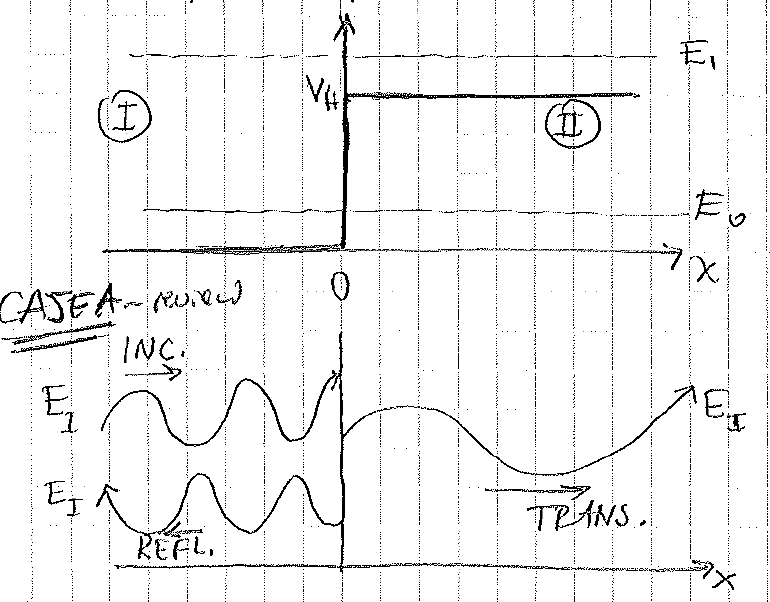
\includegraphics[width=4in]{images/qm/step-barrier-caseA.png}
    \caption{Simple Step Barrier Diagram, E$>$V}
\end{figure}


Quantum mechanically, in case A, it would transmit and/or reflect. Intuitively, in this case we would get $E_{\mathrm{reflected}} = E_{\mathrm{incoming}}$ (thus reflecting with the same wavelength), as well as a transmitted wave with $E_{\mathrm{trans}} < E_{\mathrm{incoming}}$ (thus transmitted wave with wavelength larger than the incoming one). 

\begin{itemize}
\item

Region I: 
\eqn{ -\frac{\hbar^2}{2m} \ppsipxn2 = E_1 \psi, E_1 = \frac{\hbar^2 k_1^2}{2m} }
\eqn{ \ppsipxn2 + k_I^2 \psi = 0 \Rightarrow \psi_I = A e^{ik_1x} + B e^{-ikx_1x}  }
Region II:
\eqn{ -\frac{\hbar^2}{2m} \ppsipxn2 + V_H \psi = E_1 \psi  }
\eqn{ \ppsipxn2 + k_2^2 \psi = 0 \Rightarrow \psi_{II} = C e^{ik_2 x} + D e^{-ik_2 x} }
in which $k_2^2 = \frac{2m (E_1 - V_H)}{\hbar^2}$, or $E_1  = \frac{\hbar^2 k_2^2}{2m} + V_H = KE + PE$. 

In this problem, $\psi_{II}$ is the transmitted wave traveling to the right, thus only the C term survives. 

\item 
BC1: $\psi(0^-) = \psi(0^+)$, thus $A+B = C$. 

BC2: $\left. \dpsidx \right|_{x=0^-} = \left. \dpsidx \right|_{x=0^+}$, thus $(A - B) k_1 = C k_2$. 

Together we can solve for B,C:
\eqn{ B = \frac{k_1 - k_2}{k_1 + k_2} A, \fsp C = \frac{2 k_1}{k_1 + k_2} A }

\item 
From math, we can write: 
\eqn{ k_1 |A|^2 = k_1 |B|^2 + k_2 |C|^2 }
\eqn{ \frac{\hbar k_1}{m} |A|^2 = \frac{\hbar k_1}{m} |B|^2 + \frac{\hbar k_2}{m} |C|^2 }
\eqn{ \Gamma_{\mbox{INC}} = \Gamma_{\mbox{REFL}} + \Gamma_{\mbox{TRANS}}  }
\eqn{ 1 = \frac{\Gamma_{\mbox{REFL}}}{\Gamma_{\mbox{INC}}} + \frac{\Gamma_{\mbox{TRANS}}}{\Gamma_{\mbox{INC}}}  =  T + R }
in which T is the transition probability/coefficient, and R is the reflection probability/coefficient defined as:
\eqn{ R = \frac{|B|^2}{|A|^2}, \fsp T = \frac{k_2 |C|^2}{k_1 |A|^2} } 

\item Case A recap: 
$\psi_1 (x) = A e^{ik_1 x} + B e^{i k_2 x}$ in which $k_1 = \sqrt{\frac{2 m E_1}{\hbar^2}}$. \\
$\psi_2 (x) = C e^{ik_2 x}$ in which $k_2 = \sqrt{\frac{2 m (E_1 - V_H)}{\hbar^2}}$. 

Apply BC, we can find the relationship between A,B,C. 

Apply conservation of flux $\Gamma_{\mbox{INC}} = \Gamma_{\mbox{REFL}} + \Gamma_{\mbox{TRANS}}$, and given $\Gamma = \rho v$ in which $\rho = |\psi|^2, v = \frac{\hbar k}{m}$, we know: 
\eqn{ \frac{\hbar k_1}{m} |A|^2 = \frac{\hbar k_1}{m} |B|^2 + \frac{\hbar k_2}{m} |C|^2 }
in which R and T are defined as:
\eqn{ R = \frac{|B|^2}{|A|^2}, \fsp T = \frac{k_2 |C|^2}{k_1 |A|^2} } 
\end{itemize}

\end{document}
